\section{Entanglement measures}\label{sec:2:entanglement-measures}
Checking whether an arbitrary state $\rho$ is entangled or not is no easy task. In fact, this problem is known to be NP-hard \cite{Gurvits_2003}.
A state $\rho_{AB} \in \mathcal{H}_A\otimes\mathcal{H}_B$ is called entangled, if it is \emph{non-separable}, that is, it cannot be expressed as a tensor product of two subsystems $\rho_A \in \mathcal{H}_A$ and $\rho_B \in \mathcal{H}_B$.
Only for specific cases - like the case of two qubits or qubit-qutrit - a simple sufficient criterion for determining the separability of a general mixed state is known:
The positive partial transpose (PPT) criterion states, that if the partial transpose of the density matrix is positive ($\rho^{\Gamma_A} > 0$ \footnote{A matrix is defined as positive (\q{positive definite}), if all eigenvalues are positive.}), the state $\rho$ is separable \cite{Horodecki_2009,Plenio_2005a}. In other words, if $\rho^{\Gamma_A}$ has negative eigenvalues, $\rho$ is guaranteed to describe an entangled state.
The inverse is true, if and only if the dimension of $\rho_A\otimes\rho_B$ is $2\times2$ or $3\times2$ \cite{Horodecki_2009} - otherwise, only having non-negative eigenvalues doesn't necessarily result in an unentangled system (such states are called \q{bound states}).
The partial transpose with respect to a subsystem $i$ can be understood in the same way as the partial trace, where the operation (in this case the transform) is performed only on indices corresponding the subsystem $\rho_i$.
To see the necessity of the PPT criterion, consider a separable mixed state $\rho$, which can be generally expressed as 
\begin{equation}\label{eq:2:separable-state}
  \rho = \sum p_i \rho_{A}^i\otimes\rho_{B}^i .
\end{equation}
The partial transpose is in this case trivial:
\begin{equation}
  \rho^{\Gamma_A} = \sum p_i (\rho_{A}^i)^T \otimes \rho_{B}^i .
\end{equation}
Since the transpose preserves eigenvalues, the transposed subsystem $A$ is still positive $(\rho_{A}^i)^T > 0$ and describes again a valid quantum state. It follows, that $\rho^{\Gamma_A}$ is positive as well.
If somehow $\rho^{\Gamma_A}$ has any negative eigenvalues, this can only mean that the initial state $\rho$ is not separable and cannot be expressed in the form of eq. \eqref{eq:2:separable-state} and the necessity of the criterion is shown.

For quantifying entanglement in a more precise way, a mathematical quantity called \emph{entanglement measure} can be used. A good measure should be able to capture the essential features of entanglement. One can axiomatically state what properties such a measure $E(\rho)$ should have \cite{Plenio_2005a,Horodecki_2009}:
\begin{description}
  \item[Normalization] An entanglement measure should be a mapping from densities to real positive values between 0 and 1:
  \begin{equation}
    \rho \rightarrow E(\rho) \in \mathbb{R}^+
  \end{equation}
  where usually the maximally entangled state has $E=1$.
  \item[Monotonicity under LOCC] $E$ should not increase under local operations and classical communications. This is the most important postulate for an entanglement measure and often cited as the \textit{only} required postulate.
  \item[Vanishing on separable states] $E(\rho)=0$ if $\rho$ is separable
  \item[] Often one finds additional properties useful like \textit{convexity} $E(\sum p_i \rho_i) \leq \sum p_i E(\rho_i)$ or (full) \textit{additivity} $E(\rho \otimes \sigma) = E(\rho) + E(\sigma)$.
\end{description}
A function that satisfies the most important of these conditions is often called an \textit{entanglement monotone}.

The \emph{negativity} $\mathcal{N}$ is such an entanglement monotone \cite{Vidal_2001,Plenio_2005a} that used the PPT criterion to determine if a state is entangled or not. It is defined as 
\begin{equation}\label{eq:2:negativity}
  \mathcal{N} = \frac{\norm{\rho^{\Gamma_A}}_1 - 1}{2}
\end{equation}
where $\norm{A}_1 = \tr\abs{A} = \tr \sqrt{A^\dagger A}$ is the trace norm. The negativity however is not additive and a more suitable and widely used entanglement measure is the \emph{logarithmic negativity} \cite{Plenio_2005,Horodecki_2009,Plenio_2005a}
\begin{equation}\label{eq:2:logarithmic-negativity}
  E_N(\rho) = \log_2\norm{\rho^{\Gamma_A}}_1 .
\end{equation}
The monotonicity of the logarithm implies, that $E_N$ is an entanglement monotone as well.
Furthermore, for the calculations it does not matter which subsystem is transposed.

\begin{proposition}
  a) The partial transpose w.r.t. subsystem $A$ is equal to the transposed partial transpose w.r.t. subsystem $B$: $\rho^{\Gamma_A} = (\rho^{\Gamma_B})^T$. 
  b) The trace norms of partially transposed density operators w.r.t. any subsystem are equal: $\norm{\rho^{\Gamma_A}}_1 = \norm{\rho^{\Gamma_B}}_1$.
\end{proposition}
\begin{proof}
  a) A general density matrix $\rho$ can be expressed as
  \begin{equation*}
    \rho = \sum_{i,j,k,l} \rho_{ij,kl} \ketbra{i}{j}_A\otimes\ketbra{k}{l}_B
  \end{equation*}
  The partial transpose with respect to subsystem $B$ is then defined as 
  \begin{equation*}
    \rho^{\Gamma_B} \equiv \sum_{i,j,k,l} \rho_{ij,kl} \ketbra{i}{j}_A\otimes\left(\ketbra{k}{l}_B\right)^T = \sum_{i,j,k,l} c_{ij,kl} \ketbra{i}{j}_A\otimes\ketbra{l}{k}_B
  \end{equation*}
  The complete transpose of this is
  \begin{equation*}
    (\rho^{\Gamma_B})^T = \sum_{i,j,k,l} \rho_{ij,kl} \left(\ketbra{i}{j}_A\right)^T\otimes\left(\ketbra{l}{k}_B\right)^T = \sum_{i,j,k,l} c_{ij,kl} \ketbra{j}{i}_A\otimes\ketbra{k}{l}_B \equiv \rho^{\Gamma_A}
  \end{equation*}
  b) Clear by a) and by using \cref{lemma:trace-norm-hermitian} and the fact that the eigenvalues of a square matrix $A$ and $A^T$ are equal.
\end{proof}

The logarithmic negativity is very easy to calculate compared to other entanglement measures. It is enough to compute the square root of the eigenvalues of $(\rho^{\Gamma})^\dagger \rho^{\Gamma}$ or the absolute sum of the eigenvalues of $\rho^{\Gamma}$.
For practical and numeric calculations it is often more easy and stable to take a single eigenvalue than the need to compute the sum of multiple. 
For all numerical calculations in this thesis, I therefore opt for an alternative way to compute the logarithmic negativity.

\begin{lemma}\label{lemma:trace-norm-hermitian}
  The trace norm $\norm{A}_1 \equiv \tr \sqrt{A^\dagger A}$ of a hermitian matrix $A$ is equal to the sum of the absolute eigenvalues of $A$.
\end{lemma}
\begin{proof}
  This can be immediately seen by the spectral theorem:
  \begin{equation*}
    \tr \sqrt{A^\dagger A} = \tr \sqrt{A^2} = \tr{U\sqrt{\diag(\lambda_1, \dots)^2}U^\dagger} = \sum_i \sqrt{\lambda_i^2} = \sum_i \abs{\lambda_i}.
  \end{equation*}
\end{proof}

\begin{proposition}\label{proposition:negativity}
  The negativity eq. \eqref{eq:2:negativity} is given as the absolute sum of all negative eigenvalues of $\rho^{\Gamma}$: 
\begin{equation}
    \mathscr{N}(\rho) \equiv \frac{\norm{\rho^{\Gamma}}_1 - 1}{2} = \abs{\sum_{\lambda_i < 0} \lambda_i}.
\end{equation}
\end{proposition}
\begin{proof}
  The proof is in parts given by Vidal and Werner \cite{Vidal_2001}. It is known that the density matrix is hermitian: $\rho = \rho^\dagger$. Using \cref{lemma:trace-norm-hermitian}, the trace norm of the density matrix is is given as $\norm{\rho}_1=\sum \lambda_i = \tr \rho = 1$. The partial transpose $\rho^{\Gamma}$ obviously also satisfies $\tr \rho^{\Gamma} = 1$ but might have negative eigenvalues. Since $\rho^{\Gamma}$ is still hermitian, the trace norm is given by
  \begin{equation*}
    \norm{\rho^{\Gamma}}_1 = \sum_i\abs{\lambda_i} = \sum_{\lambda_i \ge 0} \lambda_i + \sum_{\lambda_i < 0} \abs{\lambda_i} = \sum_i \lambda_i + 2\sum_{\lambda_i < 0} \abs{\lambda_i} = 1 + 2\sum_{\lambda_i < 0} \abs{\lambda_i} ,
  \end{equation*}
  where in the last step $\sum \lambda_i = \tr \rho^{\Gamma} = 1$ was used. The negativity can be defined as $\mathscr{N}(\rho) = \abs{\sum_{\lambda_i < 0} \lambda_i}$ and the statement is shown.
\end{proof}
\begin{remark}
  The PPT criterion states, that if $\rho^{\Gamma}$ has negative eigenvalues, the state $\rho$ is entangled. The negativity uses this criterion for a quantification of entanglement. This proposition makes sense of the name \textit{negativ}ity.
\end{remark}

Calculating the logarithmic negativity of the evolved state eq. \eqref{eq:2:evolved-state}, it is possible to quantify how the entanglement behaves in time. A straight forward computation following the calculation methods established above yields (for detailed calculations see appendix \ref{apx:E_N-exemplary})
\begin{equation}\label{eq:2:entanglement-dynamics-parallel}
  E_N(\ketbra{\psi(t)}) = \log_2\left(1 + \abs{\sin \Delta\phi}\right) .
\end{equation}
It is interesting to see, that the maximum entanglement $E_N = 1$ is reached for $\Delta\phi = 2\pi k \pm \pi/2, \, k\in\mathbb{Z}$ and no entanglement ($E_N=0$) is measurable for $\Delta\phi = k\pi$. This result aligns with the previous observations by demanding that the evolved state eq. \eqref{eq:2:evolved-state} is separable.
The complete entanglement dynamics are shown in \cref{fig:2:entanglement-dynamics}.
\begin{figure}[!htbp]
  \centering
  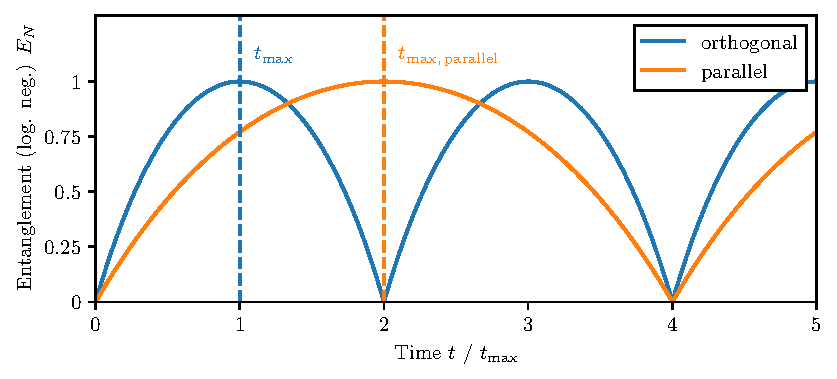
\includegraphics[width=\textwidth]{./../figures/ideal-entanglement/EN-time.pdf}
  \caption{Entanglement dynamics quantified by the logarithmic negativity for two different orientations of the spatial superpositions. The parallel orientation was considered in this chapter (see eq. \eqref{eq:2:entanglement-dynamics-parallel}), the \q{orhtogonal} one in Ref. \cite{Pedernales_2023}. The time of maximum entanglement $t_\mathrm{max}$ for the orthogonal configuration is reached after $t_\mathrm{max} = 4\pi\hbar L^3 / (G M_A M_B \Delta x^2) \simeq 129\si{ms}$.}
  \label{fig:2:entanglement-dynamics}
\end{figure}
The time $t_\mathrm{max,\,parallel}$ at which the entanglement is maximal (for the first time) can be calculated by using the definition of $\Delta\phi$ from eq. \eqref{eq:2:definition-delta-phi} as
\begin{equation}\label{eq:2:t-max-parallel}
  t_\mathrm{max,\,parallel} = \frac{8 \pi L^3\hbar}{G M_A M_B (\Delta x)^2} .
\end{equation}
In \cref{fig:2:entanglement-dynamics} the entanglement dynamics for a different orientation considered in Ref. \cite{Pedernales_2023} is also shown. 
There, the superpositions are aligned in the same line as the direct connection between the masses (\q{orthogonal} to the parallel configuration before), maximizing the differences in distances between them and thus creating entanglement faster. This expected behavior can be well seen in \cref{fig:2:entanglement-dynamics}: The time $t_\mathrm{max}$ until the maximum entanglement is reached, is precisely by a factor of $2$ faster than in the here considered parallel configuration \cite{Pedernales_2023}. 
For a practical experiment, this suggests that using the orthogonal orientation could be beneficial and would require shorter coherence times for the superpositions.
To give an estimate, consider two identical silica spheres with a density of $\rho=2648\si{kg/m^3}$ with a radius of $R=10^{-5}\si{m}$, a separation of $2L = 4R$ and a superposition size $\Delta x = 100\si{nm}$ (which is realistic considering theoretical sizes of up to micrometers \cite{Bose_2017}), the maximum entanglement is reached after about $t_\mathrm{max} \approx 129\si{ms}$ which is a quite long coherence time and challenging experimentally.